\documentclass[10pt]{article}
\usepackage{titling} % Customize the title
\usepackage[utf8]{inputenc}
\usepackage{eso-pic}
\usepackage{charter}
\usepackage[margin=1in]{geometry}
\usepackage{amssymb,pdfpages,fancyhdr,subcaption,graphicx,hyperref,float,outlines,amsmath,gensymb}
\usepackage{listings}
\usepackage{parskip}
\usepackage{multicol} % Added the multicol package
\usepackage{booktabs}
\usepackage{graphicx}
\usepackage{subcaption}
\usepackage{multirow}
\usepackage{listings}
\usepackage{colortbl}

% Define colors for code highlighting
\definecolor{codegreen}{rgb}{0,0.6,0}
\definecolor{codegray}{rgb}{0.5,0.5,0.5}
\definecolor{codepurple}{rgb}{0.58,0,0.82}
\definecolor{backcolour}{rgb}{0.95,0.95,0.92}

% Define settings for Python code
\lstdefinestyle{mystyle}{
    backgroundcolor=\color{backcolour},
    commentstyle=\color{codegreen},
    keywordstyle=\color{blue},
    numberstyle=\tiny\color{codegray},
    stringstyle=\color{codepurple},
    basicstyle=\ttfamily\footnotesize,
    breakatwhitespace=false,
    breaklines=true,
    captionpos=b,
    keepspaces=true,
    numbers=left,
    numbersep=5pt,
    showspaces=false,
    showstringspaces=false,
    showtabs=false,
    tabsize=2
}

\lstset{style=mystyle}

\title{\textbf{4M17 Coursework \#2 \\ Optimisation Algorithm Performance Comparison}}
\author{\textbf{Candidate No: 5730E}}

\begin{document}
\maketitle
\begin{multicols}{2}\begin{figure}[H]
    \centering
    \begin{subfigure}{0.49\textwidth}
        \centering
        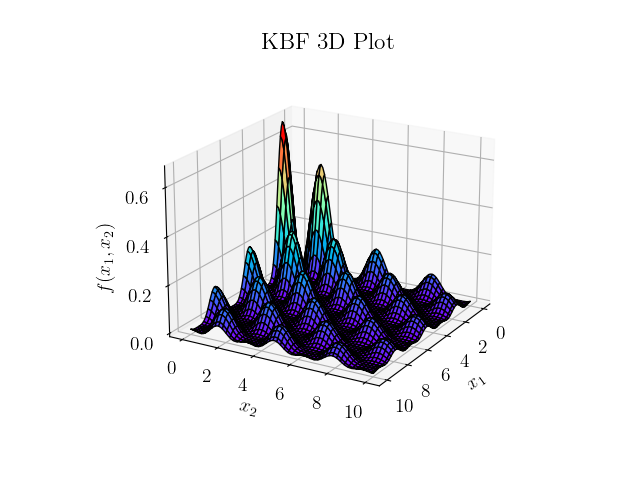
\includegraphics[width=\textwidth]{../figures/KBF/KBF_surf.png}
        \caption{Surface plot.}
        \label{fig:KBF_surf}
    \end{subfigure}
    \begin{subfigure}{0.49\textwidth}
        \centering
        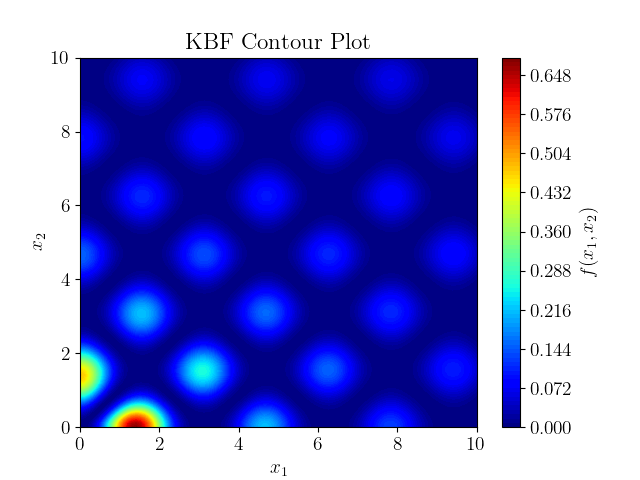
\includegraphics[width=\textwidth]{../figures/KBF/KBF_contour.png}
        \caption{Contour plot.}
        \label{fig:KBF_contour}
    \end{subfigure}
        \captionsetup{justification=centering}
        \caption{Two-dimensional visualisation of the Keane's Bump Function, (KBF).}
        \label{fig:KBF_2D}
\end{figure}

\section{Abstract}
This report conducts a comparative analysis of two optimisation algorithms applied to minimise Keane's Bump Function, (KBF). In particular, the study focuses on a Continuous Genetic Algorithm, (CGA), as well as an alternative algorithm not covered in the lectures: Parallel Tempering, (PT). 

\section{Problem Setup: Keane's Bump Function}

To compare the performances of the two algorithms, the Keane's Bump Function, (KBF), is used as the objective function. In particular, the n-dimensional constrained optimisation problem is defined as the maximisation of:

\begin{equation}
    f(\mathbf{x}) = \left| \frac{\sum_{i=1}^{n} (\cos(x_i))^4 - 2\prod_{i=1}^{n} (\cos(x_i))^2}{\sqrt{\sum_{i=1}^{n} i \cdot x_i^2}} \right|
    \label{eq:KBF_cost}
\end{equation}
\begin{equation}
    \begin{aligned}
        \text{subject to} \quad & 0 \leq x_i \leq 10 \quad \forall i \in \{1, \dots, n\} \\
        & \quad \prod_{i=1}^{n} x_i > 0.75 \\
        & \quad \sum_{i=1}^{n} x_i < \frac{15n}{2}
    \end{aligned} 
    \label{eq:KBF_constraints}
\end{equation}

The two-dimensional form of the function has been plotted in Figure \ref{fig:KBF_2D}. Some notable properties are as follows:

\begin{itemize}
    \item The function is undefined at the origin, (0, 0). This is due to the division by zero in the denominator of Equation \ref{eq:KBF_cost}. Otherwise, the function is continuous and differentiable everywhere.
    \item The function is highly multi-modal. Its global maximum is located on the constaint boundary $x_{n}=0$, where $x_n$ denotes the final variable in the n-dimensional space. However, there are many local maxima located inside the feasible region, all of which have quite similar amplitudes.
    \item The function is nearly symmetric about the line $x_1=x_2$. This stems from its construction in \ref{eq:KBF_cost}, using the sums of squared, symmetric terms, $x_i^2$, $(\cos(x_i))^2$, and $(\cos(x_i))^4$. This results in some invariance regarding the order of the input variables. Overall, the peaks consistently manifest in pairs, yet there is a notable pattern wherein one peak always surpasses its counterpart in magnitude.
\end{itemize}

Given the above properties, the KBF is a challenging function to optimise. The presence of multiple, similar-amplitude local maxima makes it difficult for an optimisation algorithm to converge to the global maximum. On the other hand, all control variables share the same nature, (continuous variables), and exhibit identical scales. Additionally, all constraints are of the inequality type, and the feasible space is non-disjoint.

The problem becomes more complicated with the inclusion of the constraints outlined in \ref{eq:KBF_constraints}. Figure \ref{fig:KBF_Feasible} illustrates the resulting feasible region carved out of the original function space. Notably, the contstraint boundaries are non-linear. The problem complexity is additionally excaberated by the presence of multiple optima along the constraint boundaries, including the global maxima that we seek to identify.

These properties make the KBF a suitable candidate for the comparative analysis of the two optimisation algorithms, as discussed in the previous work \cite{ELBELTAGY1999639}.

\begin{figure}[H]
    \centering
    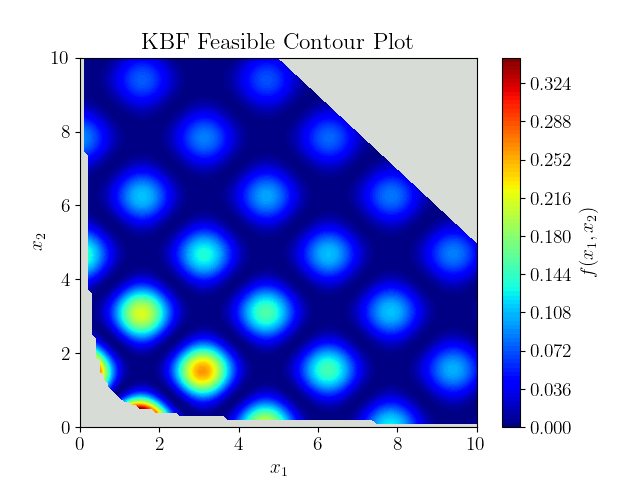
\includegraphics[width=0.48\textwidth]{../figures/KBF/KBF Feasible_contour.png}
    \captionsetup{justification=centering}
    \caption{Feasible region carved out from the two-dimensional visualisation of the Keane's Bump Function, (KBF).}
    \label{fig:KBF_Feasible}
\end{figure}

\section{The Continuous Genetic Algorithm (CGA)}
\label{sec:CGA}

The discrete nature of the GA presented in \cite{parks2023geneticalgorithms} makes it unsuitable for the optimisation of the KBF. An implementation of a Continuous Genetic Algorithm, (CGA), is used instead, which lends itself better to the problems presented in \ref{eq:KBF_cost}-\ref{eq:KBF_constraints}.

The CGA, a technique inspired by natural selection and genetics, presents itself as particularly well-suited to tackling challenges associated with multiple local optima. Furthermore, the algorithm lends itself well to parallelisation with low implementation effort, and offers ample opportunities for modifications and adaptations, supported by a rich body of literature on the subject.

The primary difference between the CGA and the GA in \cite{parks2023geneticalgorithms} is the representation of individuals, (solutions of the state space), within the population. Rather than representing an individual as a vector of binary values or bits, (0s and 1s), the CGA uses a real-valued vector of floating-point numbers to represent each individual, as discussed in \cite{PGA}. This allows for a direct representation of the problem, and eliminates the need for a decoding function, which reduces overhead in function evaluations.

This adjustment marks a significant departure from conventional GAs, aligning the algorithm more closely with Evolution Strategies (ES), another member of the evolutionary algorithms family presented in \cite{salimans2017evolution}. However, the algorithm presented in \ref{sec:CGA_implementation} is still classified as a GA in accordance with the differences presented in \cite{10.1007/BFb0029787}, given that mutation does not serve as the primary search mechanism for exploring the state space. Instead, it functions as a non-adaptive, background operator.

\subsection{Implementation}
\label{sec:CGA_implementation}

In accordance with the terminology presented in \cite{parks2023geneticalgorithms}, a vector solution of the state space will be referred to as an \textit{individual} or \textit{chromosome}. Correspondingly, a collection of such individuals arranged in a matrix format will be denoted as a \textit{population}. Each individual is delineated as an $n \times 1$ vector of real-valued (floating-point) numbers, where $n$ signifies the number of variables in the state space. The population itself is represented as a $m \times n$ matrix, where $m$ designates the count of individuals in the population. This count is explicitly defined as a hyperparameter within the codebase: %placeholder

\begin{figure}[H]
    \centering
    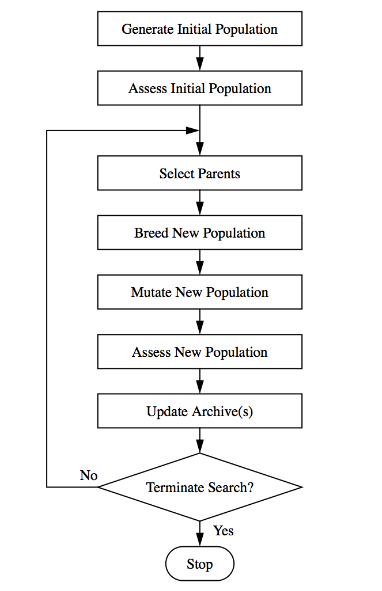
\includegraphics[width=0.48\textwidth]{../figures/Permanent Images/Flowchart.png}
    \captionsetup{justification=centering}
    \caption{A flowchart depicting the CGA process, taken from \cite{parks2023geneticalgorithms}.}
    \label{fig:GAprocess}
\end{figure}

The CGA process is outlined in Figure \ref{fig:GAprocess}. Notably, three selection strategies and two mutation procedures were deliberately implemented to harness the flexibility inherent in the CGA, tailoring it to the optimisation challenges posed by the KBF. The subsequent section, \ref{sec:CGA_selection_mutation}, elucidates the selection method and mutation procedure choices that form the basis of the forthcoming comparison.

The CGA can be can be finely tuned for a specific objective function by modifying its fitness function, which assesses the quality of an individual. The management of constraints is woven into the selection process, as outlined below.

\subsubsection{Initialisation}

The population is initialised with random values uniformly distributed within the range of 0 to 10, which represents the bounds of the state space, encompassing both feasible and infeasible values. This population comprises 250 individuals, as defined by the \textit{POPULATION\_SIZE} hyperparameter. 

\subsubsection{Parent Selection}

Three selection methods were implemented: proportional selection, tournament selection, and stochastic remainder selection without replacement (SRS). The hyperparameter governing the quantity of parents chosen, denoted as \textit{NUM\_PARENTS}, is established at 25\% of the population size, (rounded down to the nearest even number to facilitate the creation of parent pairs).

Another important aspect of the selection process is the handling of constraints. In particular, the selection process is repeated until only feasible individuals are selected. Infeasible individuals are simply not chosen as parents, a strategy advised by \cite{parks2023geneticalgorithms}, which was deemed suitable considering that the feasible space is non-disjoint, and the constraints are of the inequality type.

\textbf{\underline{Proportional Selection}}

The probability of an individual being selected for mating is proportional to its fitness:
\[
    P_i = \frac{f_i}{\sum_{i=1}^{n} f_i}
\]
Here, \(f_i\) denotes the fitness of the \(i\)th individual. This is the simplest selection method, and is implemented in accordance with the theory presented in \cite{parks2023geneticalgorithms}.

As noted in \cite{parks2023geneticalgorithms}, this approach is susceptible to high variance in individual selection, primarily because there is no assurance of choosing the optimal individual. Alternatively, the following two procedures show greater potential, incorporating a degree of determinism into the selection process.

However, it would be premature to disregard the proportional selection method. There is a chance that the determinism inherent in the other two methods could negatively impact the KBF optimisation process. A notable degree of stochasticity may improve the algorithm's effectiveness in exploring the search space, which may prove vital given the multi-modal nature of the KBF.

\textbf{\underline{Tournament Selection}}

As outlined in \cite{parks2023geneticalgorithms}, this strategy involves taking a small subset of the population, and selecting the top two individuals with the highest fitness. This is repeated until the required number of parents is achieved. Selection pressure can then be adjusted by varying the size of the subset, controlled by the \textit{TOURNAMENT\_SIZE} hyperparameter.

This is a popular selection method, as it is simple to implement, and is known to perform well in practice. It can be improved by including some of the concepts presented in \cite{Miller1995GeneticAT}, however, these have been avoided to reduce the complexity of the algorithm's implementation.

\textbf{\underline{Stochastic Remainder Selection}}\\\vspace{0.5mm}
\textbf{\underline{\hspace{-0.5mm}without Replacement (SRS)}}

This strategy draws inspiration from \cite{parks2023geneticalgorithms}. Specifically, a group of chosen individuals is curated by generating an expected number of copies for each individual, denoted as: 
\[E_i = N * P_i\]
Here, \(N\) represents the population size, and \(P_i\) is elucidated above in the context of proportional selection. The anticipated number of duplicates is subsequently divided into an integer part, \(I_i = \lfloor E_i \rfloor\), and a remainder, \(R_i = E_i - I_i\). 

The integer part is used for deterministic selection of individuals. The $i$th indivdual is selected $I_i$ times. Subsequently, the remained, $R_i$, is then used to stochastically augment the collection of individuals until the required number of parents is achieved. This is done by selecting the $i$th individual with a probability of $R_i$.

The discussion in \cite{parks2023geneticalgorithms} highlights that this approach appears to yield superior performance, ascribed to the inclusion of a degree of determinism in the selection criteria. Nevertheless, it remains worthwhile to evaluate the performance of the other two methods, as they might present distinct advantages within the framework of the KBF.

\subsubsection{Mating Procedure}

Similarly, two mating procedures have implemented: crossover and heuristic crossover. The entire population is replaced by offspring, bred from two randomly allocated parents from the pool of selected parents.

\textbf{\underline{Crossover}}

The crossover procedure adheres to the principles detailed in \cite{parks2023geneticalgorithms}. Initially, a crossover point is randomly chosen. Genes from the first parent are incorporated into the offspring until this point, beyond which genes from the second parent take their place. Specifically, the sequencing of the parents is governed by the probability specified by the hyperparameter \textit{CROSSOVER\_PROB}.

\textbf{\underline{Heuristic Crossover}}

Heuristic crossover is presented in \cite{Michalewicz_2011}. By this variation, a random number $\beta$ in the interval $[0, 1]$ is generated. The genes of the offspring are then determined as a blend of the original two parents, $p_1$ and $p_2$, as follows:
\[
    o_i = \beta (p_{1i} - p_{2i}) + p_{2i}
\]
With this inspiration in mind, heuristic crossover was implemented in the CGA. Specifically, the sequence of parents in the above formula is determined by the \textit{CROSSOVER\_PROB} hyperparameter, aligning with the approach used previously in the original crossover procedure.

A crucial factor to bear in mind is that certain offspring may be produced outside the feasible region. This implementation deviates from the recommendation in \cite{Michalewicz_2011} by not outright rejecting these offspring during the mating procedure. Rather, they are simply excluded from consideration as parents in the subsequent selection process.

The decision to incorporate this mutation procedure stems from the continuous nature of the state space. While the conventional crossover methods may be well-suited to binary representations, a more intuitive approach emerges when grappling with real-valued variables - using a blend of characteristics from both parents.

Moreover, the use of the heuristic crossover method aims to address previous limitations associated with standard crossover. Unlike conventional crossover, which confines offspring values to those of the parents, blending permits the generation of offspring beyond the parent values, allowing for potentially new information. This feature may prove particularly advantageous in the context of the KBF, enhancing the algorithm's capability to navigate the search space adeptly and thoroughly explore local optima.

An additional noteworthy observation is that the introduction of $\beta$ serves to bring the CGA into closer alignment with Evolutionary Strategies (ES). This resemblance becomes evident as the formulation above bears some similarity to the intermediate recombination strategy outlined in \cite{salimans2017evolution}. Nevertheless, it is essential to emphasise, as mentioned earlier, that mutation does not serve as the primary search mechanism in the CGA. Consequently, the CGA can still be appropriately categorised as a GA, as per the classification seen in \cite{10.1007/BFb0029787}.

\subsubsection{Mutation}

The mutation procedure proposed by \cite{PGA} involves perturbing a gene within a chromosome by a normally distributed random number with a mean of zero and a standard deviation of $\sigma$. However, the effectiveness of this procedure is constrained by the selection of $\sigma$ as an additional hyperparameter, necessitating careful tuning. 

Instead, a simpler approach was adopted, where genes within the population have an probability, given by the mutation rate, of being reset to a random value drawn from a uniform distribution within the confines of the state space, mirroring the initialisation procedure.

\subsubsection{Evaluation}

The population is then evaluated, and the individuals are ranked in order of fitness. Here, the fitness is defined as the negative of the KBF cost function, outlined in \ref{eq:KBF_cost}. This is done to align the algorithm with the maximisation of the KBF.

\subsubsection{Termination}

For this section of the report, the algorithm terminates after a maximum number of iterations, (defined as a hyperparameter). A more stringent convergence criterion is adopted for the comparison between the two algorithms in Section \ref{sec:CGA_QEG_comparison}. The individual with the lowest fitness value is then returned as the optimal solution to the optimisation problem.

\subsection{Tuning the CGA Hyperparameters}
\label{sec:CGA_selection_mutation}

Given the flexibility of the CGA, multiple selection methods and mutation procedures were implemented within the codebase, as discussed previously. These are then selected as hyperparameters within the script, %placeholder
to take advantage of the flexibility offered by the CGA. 

To choose a selection method and mutation procedure going forwards into the main comparison of this report, code %placeholder
was used as a platform for exploartion. Each selection method and mutation procedure was evaluated over 10 and 100 iterations, with a constant mutation rate of 0.05, and a crossover probability of 0.7. The number of parents was established at 25\% of the population size, (rounded down to the nearest even number to facilitate the creation of parent pairs). The population size itself was set at 250, and the tournament size was similarly defined as 25\% of this.

Additional results from the initial exploration of hyperparameter tuning are detailed in the Appendix. Specifically, the final fitness values are outlined in Table \ref{tab:CGAexploration}. Further insights into the initial evolution of the population during the first 8 iterations are illustrated in supplementary figures found in Figures \ref{fig:CGA_flowchart_SRS}, \ref{fig:CGA_flowchart_proportional}, and \ref{fig:CGA_flowchart_tournament}.
\begin{figure}[H]
    \centering
    \begin{subfigure}{0.44\textwidth}
        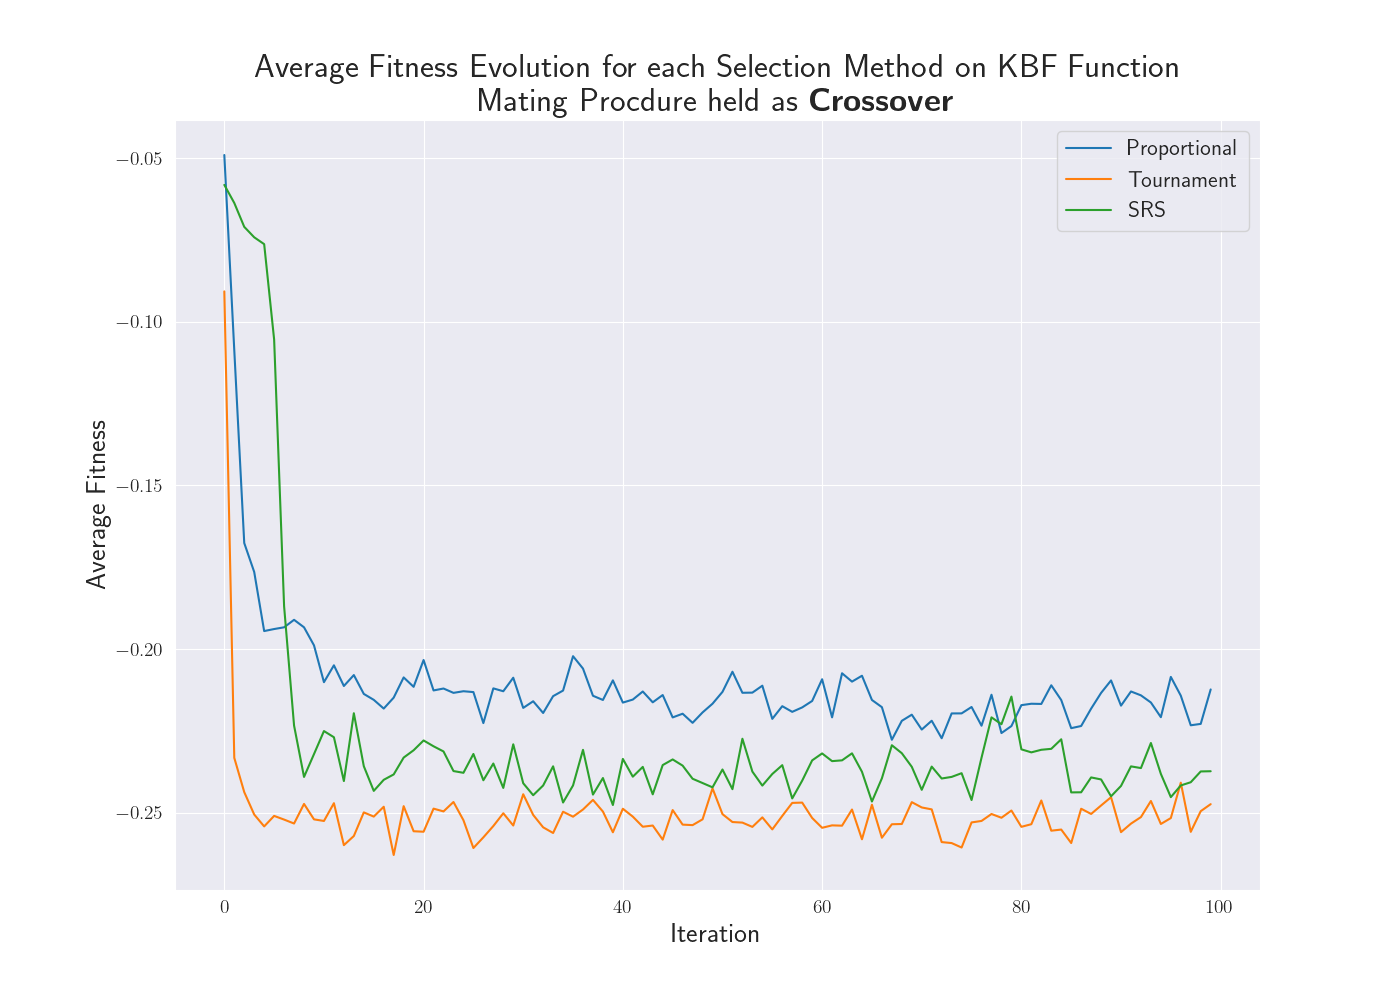
\includegraphics[width=\textwidth]{../figures/Permanent Images/Fitness_Evolution_Crossover.png}
        \caption{Mutation Procedure: Crossover}
    \end{subfigure}
    \begin{subfigure}{0.44\textwidth}
        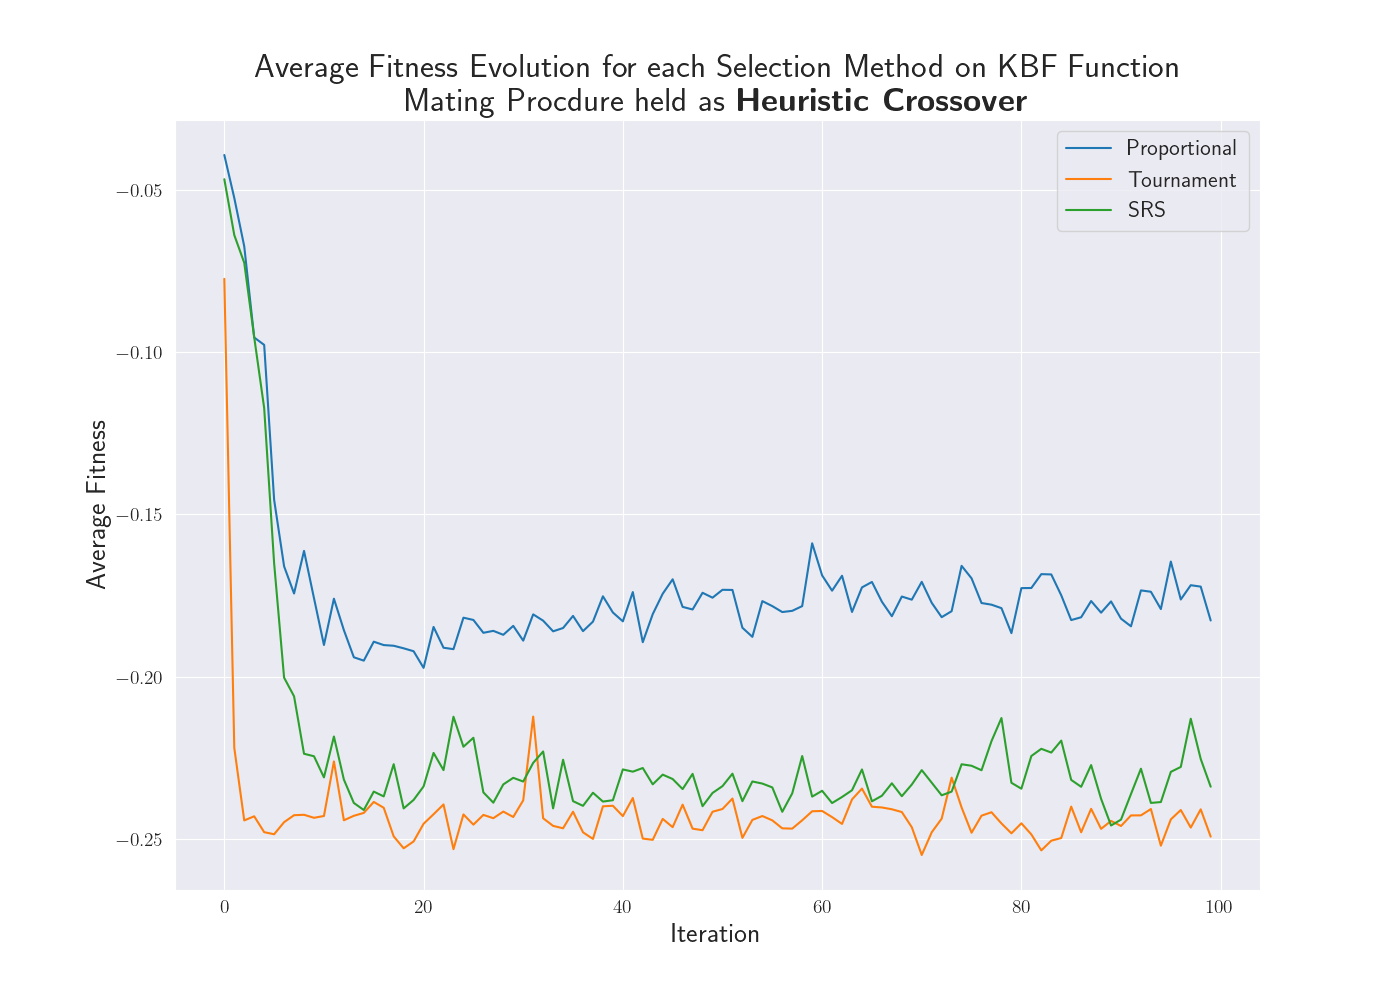
\includegraphics[width=\textwidth]{../figures/Permanent Images/Fitness_Evolution_Heuristic Crossover.png}
        \caption{Mutation Procedure: Heuristic Crossover}
    \end{subfigure}
    \captionsetup{justification=centering}
    \caption{Evolution of the average fitness values of the CGA population over 100 iterations for each of the selection methods. The results are presented for both mutation procedures: crossover and heuristic crossover. Here, the mutation rate was set to 0.05, and the crossover probability was set to 0.7.}
    \label{fig:CGA_fitness_evo}
\end{figure}

However, the most insightful conclusions can be drawn from the figures presented in \ref{fig:CGA_fitness_evo}, which illustrate the evolution of the average fitness values of the CGA population over 100 iterations for each of the selection methods. They illustrate that tournament selection seemed to outperform the other two selection methods when maximising the KBF, which is surprising given the favourable description in \cite{parks2023geneticalgorithms} regarding SRS. 

The experiment was repeated several times, yielding results that were admittedly variable, attributed to the inherent stochastic nature of the CGA. At times, the superiority of SRS over tournament selection was evident, yet proportional selection generally did not prove to perform better. Despite this variability, the outcomes exhibited sufficient consistency to justify the designation of tournament selection as the primary method for the upcoming comparison.

The observed differences in performance may be attributed to the distinct characteristics of the KBF. Tournament selection appears to demonstrate greater efficacy in navigating the search space compared to SRS, perhaps due to its less deterministic nature. This becomes particularly significant in light of the multi-modal nature of the KBF, where a certain level of stochasticity may prove essential for thorough exploration of the search space.

The findings additionally suggest that the heuristic crossover procedure consistently outperformed the standard crossover method, as evidenced by its more frequent attainment of the global maxima. 

This may be attributed to the heuristic crossover's capacity to generate offspring beyond the existing genotypes present within a generation. This attribute is especially beneficial within the framework of the KBF, enhancing the algorithm's ability to navigate the search space adeptly and systematically explore the numerous local optima.

Having cemented the selection method and mutation procedue choices as tournament selection and heuristic crossover respectively, the CGA was further tuned to optimise its performance. 

Specifically, choices for the mutation rate and crossover probability were explored. The results are presented in Figure \ref{fig:CGA_contour_rates}, which showcases two heat maps of the final fitness values after 100 iterations for the CGA using the chosen procedures. The plots are presented for both the average final fitness, as well as the final fitness of the best individual.

Notbaly, as depicted in Fig. \ref{fig:CGA_contour_tournament_Heuristic Crossover_AVG}, it is evident that an increased stochasticity of the CGA, indicated by higher crossover probabilities, leads to improved average final fitness. This aligns with expectations, as a broader and more randomly distributed population enhances the likelihood of individuals being situated in the proximity of local maxima. Consequently, a greater number of individuals within the population receive lower fitness values, a trend reflected in the observed average final fitness.

Fig. \ref{fig:CGA_contour_tournament_Heuristic Crossover_MIN} offers deeper insights. It is evident that the crossover probability stands out as the most influential hyperparameter, while the fine-tuning of the mutation rate plays less of a role in shaping the performance of the CGA. 

\begin{figure}[H]
    \centering
    \begin{subfigure}{0.46\textwidth}
        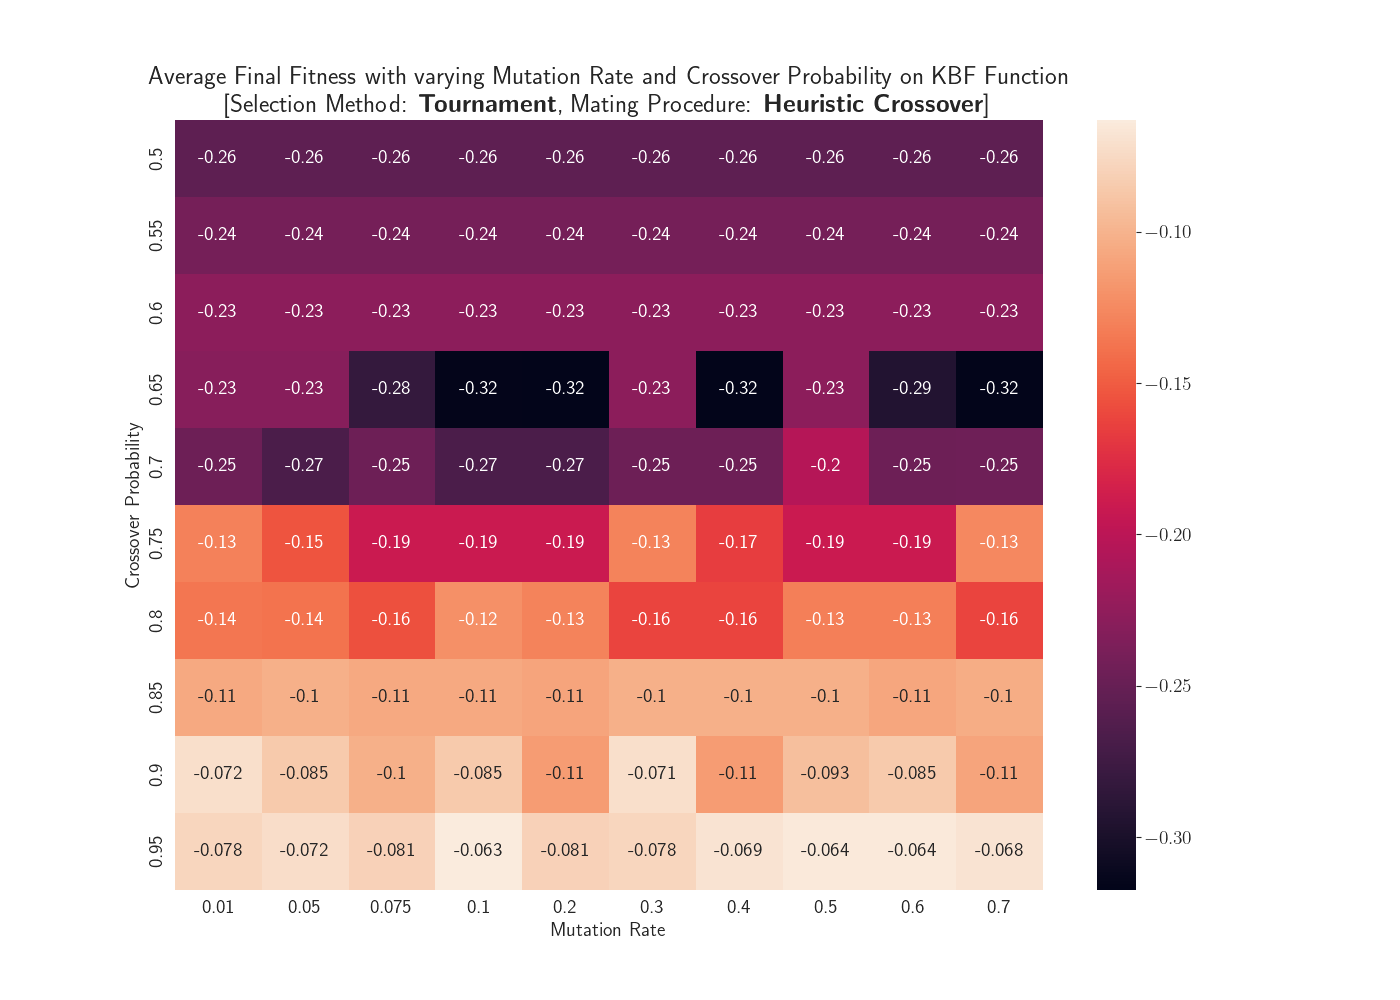
\includegraphics[width=\textwidth]{../figures/Permanent Images/AVGContour_Tournament_Heuristic Crossover.png}
        \caption{Average final fitness across entire population.}
        \label{fig:CGA_contour_tournament_Heuristic Crossover_AVG}
    \end{subfigure}
    \begin{subfigure}{0.46\textwidth}
        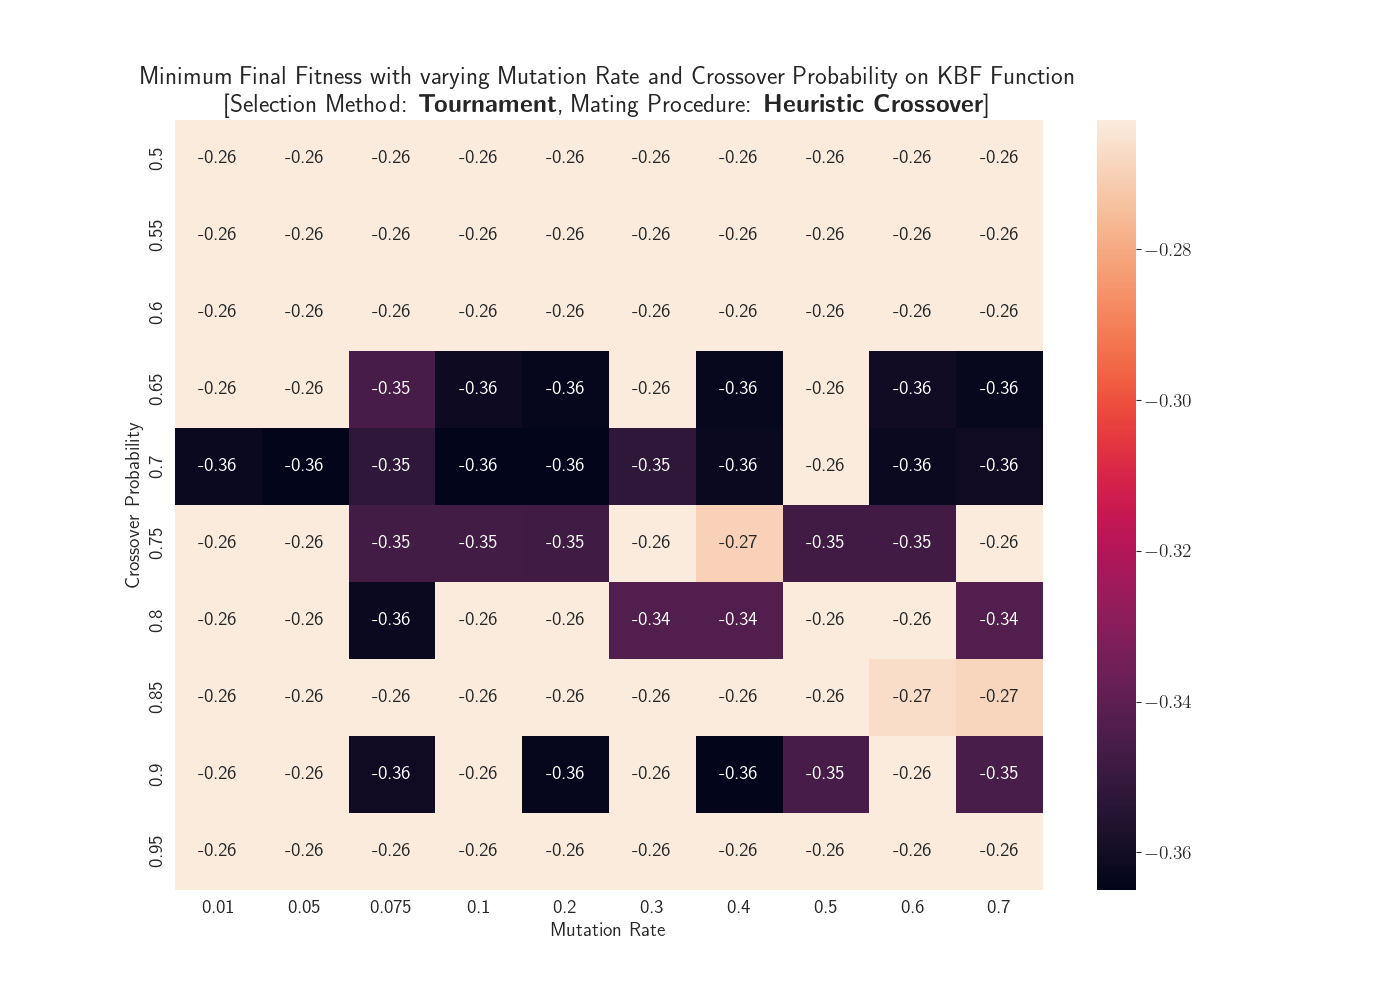
\includegraphics[width=\textwidth]{../figures/Permanent Images/MINContour_Tournament_Heuristic Crossover.png}
        \caption{Final (minimum) fitness of best individual.}
        \label{fig:CGA_contour_tournament_Heuristic Crossover_MIN}
    \end{subfigure}
    \captionsetup{justification=centering}
    \caption{Heat maps of the final fitness values after 100 iterations for the CGA using tournament selection and heuristic crossover. Here, the mutation rates and crossover probabilities were varied to assess their impact on performance.}
    \label{fig:CGA_contour_rates}
\end{figure}

\begin{figure}[H]
    \centering
    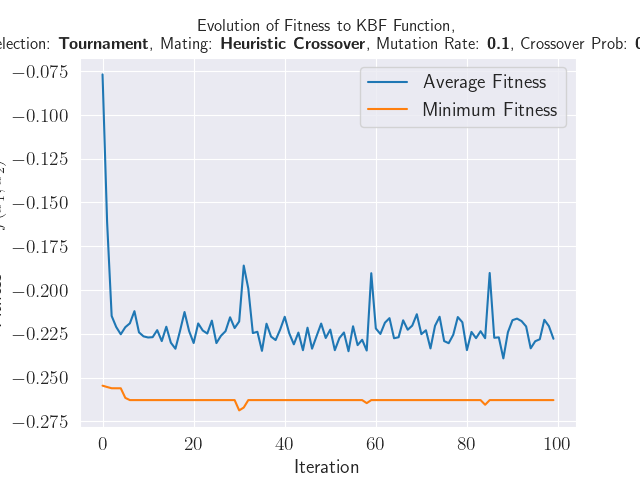
\includegraphics[width=0.48\textwidth]{../figures/Permanent Images/0.1_0.65_Fitness.png}
    \captionsetup{justification=centering}
    \caption{Evolution of the fitness values of the CGA population over 100 iterations for optimally-tuned CGA.}
    \label{fig:CGA_fitness_evo_OPT}
\end{figure}

Overall, a clear optimal set of hyperparameters emerges. Moving forward, the mutation rate is fixed at 0.1, and the crossover probability is set to 0.65. These values have proven to yield a consistently optimal performance for the algorithm, comfortably lying within the darker regions of the heat maps.

To reiterate and summarise this section of the report, the CGA is now constructed as follows:
\begin{itemize}
    \item \textbf{Selection Method:} Tournament Selection
    \item \textbf{Mutation Procedure:} Heuristic Crossover
    \item \textbf{Mutation Rate:} 0.1
    \item \textbf{Crossover Probability:} 0.65
    \item \textbf{Tournament Size:} 62
    \item \textbf{Number of Parents:} 62
    \item \textbf{Population Size:} 250
\end{itemize}

Fig. \ref{fig:CGA_fitness_evo_OPT} depicts the evolution of the fitness values over 100 iterations using the optimal hyperparameters delineated above. Note that the (minimum) fitness attributed to the best individual remains constant, because an individual within the population is stochastically initialised near the maxima that the algorithm converges to. This is less likely to occur in 8-dimensional space, where the search space is significantly larger, and the fitness of the best individual is expected to evolve more noticeably.

Fig. \ref{fig:optimal_convergence} depicts the convergence of the population to the second largest maxima over 4 and 80 iterations using the optimally-tuned CGA. Regrettably, global maximum convergence remained elusive even after 100 iterations. However, there does seem to be a discernible trend of the algorithm converging towards the second-largest maxima in Fig. \ref{fig:optimal_convergence}, offering a promising indication of progress. 

The primary challenge lies in the fact that both the first and second largest maxima are situated along the non-linear constraint boundary of the optimisation problem, posing a difficult navigational challenge.

\end{multicols}
\begin{figure}[H]
    \centering
    \begin{subfigure}{0.9\textwidth}
        \centering
        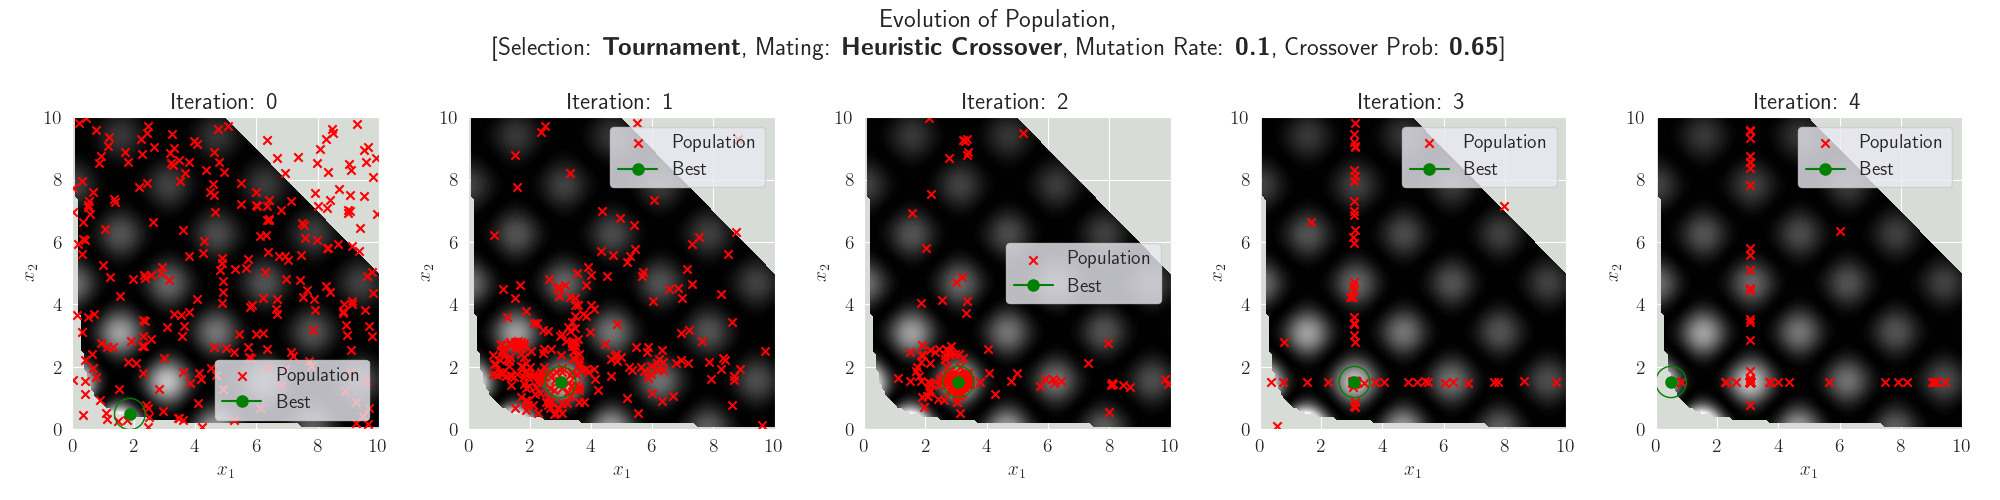
\includegraphics[width=\textwidth]{../figures/Permanent Images/0.1_0.65_Population.png}
        \caption{4 iterations.}
        \label{fig:optimal_5}
    \end{subfigure}
    \begin{subfigure}{\textwidth}
        \centering
        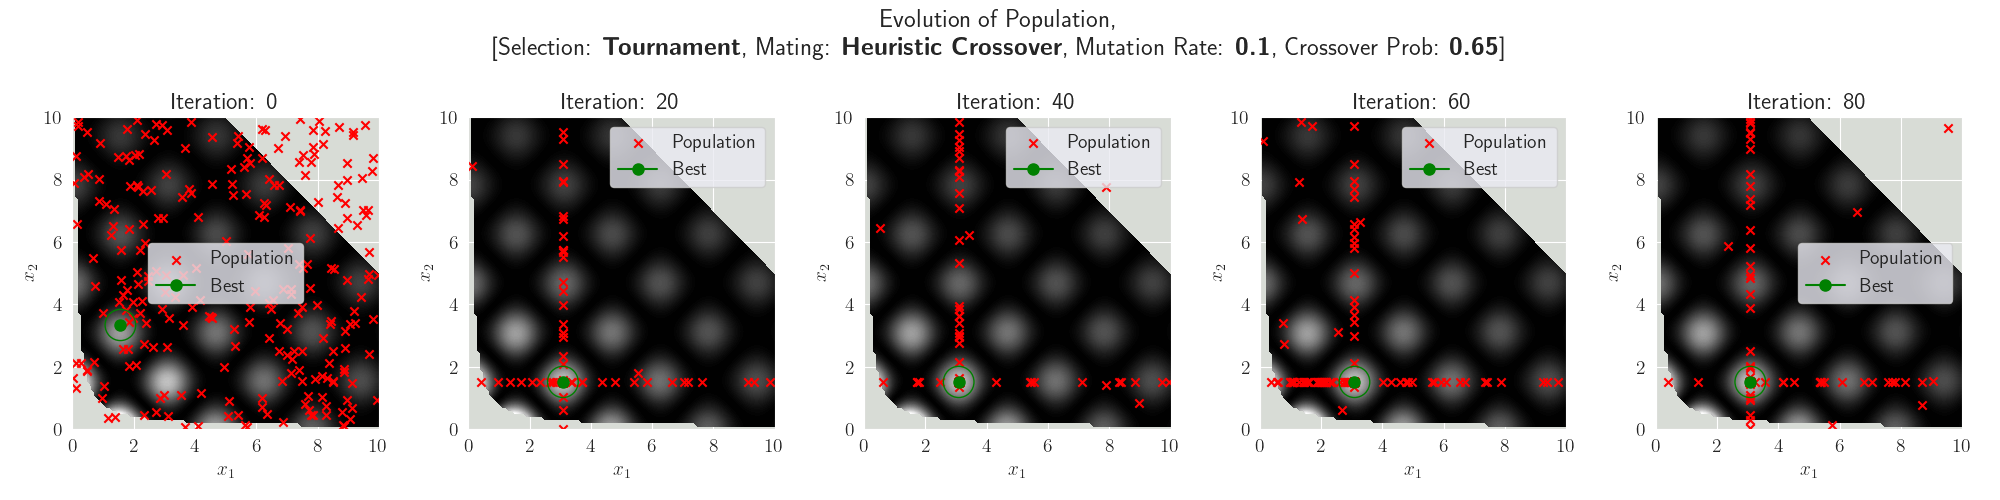
\includegraphics[width=0.9\textwidth]{../figures/Permanent Images/0.1_0.65_Population100.png}
        \caption{80 iterations.}
        \label{fig:optimat_100}
    \end{subfigure}
    \captionsetup{justification=centering}
    \caption{Evolution of the CGA population over 4 and 80 iterations using the optimal hyperparameters delineated at the end of Section \ref{sec:CGA_selection_mutation}.}
    \label{fig:optimal_convergence}
\end{figure}

\begin{multicols}{2}

\section{Parallel Tempering (PT)}
\label{sec:PT}

Having obsererved the CGA's performance and its difficulty in identifying global maxima effectively, an informed decision was made to introduce Parallel Tempering (PT) as the second algorithm for comparison.

This is a Markvo Chain Monte Carlo (MCMC) optimisation approach presented in \cite{Earl_2005}. Similar to simulated annealing, (SA), it revolves around the idea of smoothening the search space by introducing a temperature parameter, $t$. 

By incorporating a Metropolis-Hasting acceptance probability that is proportional to $\exp(1/t)$, exploration of the solution space is encouraged at high temperatures, while exploitation of the local nature of the function is facilitated at low temperatures. At high temperatures, the acceptance distribution is is smoothened out by this proportionalilty, and the algorithm is then able to explore the search space more thoroughly. As the temperature diminishes, the acceptance distribution becomes more dependent on the fitness of the proposed solution to the KBF, enabling the algorithm to explore the local nature of the function.

However, PT incorporates the novel concept of Replica Exchange Monte Carlo. Unlike SA, which operates along a single tragectory, starting with a high temperature that gradually decreases, PT maintains multiple replicas of the system at different temperatures simultaneously. Each replica explores its own solution space, and exchanges of the solutions can occur between replicas at adjacent temperature levels. This exchange mechanism enhances global exploration by facilitating the movement of solutions between replicas operating at high and low temperature. 

This parallel exploration across temperatures improves the algorithm's ability to escape local optima, providing a valuable alternative to traditional single-trajectory methods like SA. Consequently, PT could emerge as a well-suited approach for maximising the highly multi-modal KBF.

Unfortunately, this introduces an elevated computational cost, due to the management of multiple replicas and the periodic exchange of solutions. However, the potential advantages in terms of global exploration of the KBF outweigh the added computational expense. This is especially true, considering the highly parallelisable nature of PT, which may allow for even more efficient utilisation of parallel computing resources than the CGA. 

\subsection{Implementation}

PT originates from statistical physics, as extensively discussed in \cite{Earl_2005}. Therefore the following implementation draws inspiration from literature focused on sampling from complex probability distributions. 

The discourse presented in \cite{Earl_2005} emphasises a delicate trade-off between optimising MCMC sampling outcomes and minimising computational efforts. Hence, the PT implementation presented here is deliberately crafted for flexibility, offering the ability to fine-tune the algorithm, as shown in Section \ref{sec:PTtuning}.

As per the guidance in \cite{parks2023geneticalgorithmsSA}, constraints are handled by simply rejecting any proposed changes that violate the constraints. This is accomplished within the Metropolis-Hastings criterion regarding the acceptance or rejection of a proposed change. This was determined as a suitable approach, given that the feasible space is non-disjoint, and the constraints are of the inequality type.

The approach can additionally be characterised as population-based, incorporating 10 replicas in accordance with the \textit{NUM\_REPLICAS} hyperparameter. Within each replica, there are 25 chains of solutions determined by the \textit{NUM\_CHAINS} hyperparameter. Consequently, the total number of solutions being evaluated at any given time is 250, which is equivalent to the population size of the CGA.

\subsubsection{Initialisation}
The chains are initialised within the range of 0 to 1, as advised by the guidance provided in \cite{NT90-A34350}, specifically under the SA-derived solution generation framework employed in this implementation.

This range persists throughout the algorithm, until function evaluations are necessitated, at which point the \textit{scale\_up} lambda function is called to return the solution in the original state space.

Mirroring the CGA implementation, solutions were initialised without consideration for their feasibility. Whilst initialising within the feasible solution space was observed to enhance performance, this approach was deliberately omitted to ensure fair comparisons between the PT and CGA. However, the performance was notably compromised, given that solutions initialised deep within the infeasible zones of the search space faced challenges in escaping under the Metropolis-Hastings acceptance criterion.

\subsubsection{Temperature Scheduling}

A significant source of flexibility in PT lies in setting and adapting the temperatures of the replicas, as discussed in \cite{Earl_2005}. Drawing insights from the previous work of \cite{CALDERHEAD20094028} on an unrelated, yet similar problem, this was taken advantage of by parameterising the temperature schedule between 0 and 1, as follows:

\begin{equation}
    T_i = \left(\frac{i}{{N_{\text{replicas}}}}\right)^p \quad \forall i \in \{1, \dots, N_{\text{replicas}}\}
    \label{eq:PTtemp}
\end{equation}

Here, $T_i$ denotes the temperature of the $i$th replica, and $N_{\text{replicas}}$ is the total number of replicas. The exponent $p$ is a hyperparameter referred to as \textit{POWER\_TERM} that can be tuned to optimise the performance of the algorithm. 

Fig. \ref{fig:PTtemp} illustrates the influence of parameter $p$ on the temperature schedule. It intuitively demonstrates how $p$ affects the balance between exploration and exploitation. A higher value of $p$ corresponds to a slower and more gradual increase in temperature, promoting a conducive environment for exploration. A smaller value of $p$ results in a more rapid increase in temperature, encouraging exploitation of the local nature of the function.

\begin{figure}[H]
    \centering
    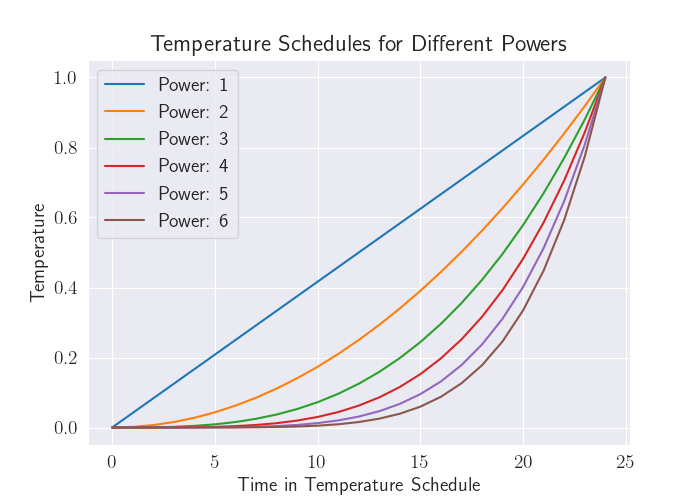
\includegraphics[width=0.48\textwidth]{../figures/Permanent Images/Power_Progression.png}
    \captionsetup{justification=centering}
    \caption{Temperature schedule \ref{eq:PTtemp} for the PT algorithm for different values of the \textit{POWER\_TERM} hyperparameter.}
    \label{fig:PTtemp}
\end{figure}

Tuning this balance is crucial for the algorithm's performance against the KBF, and is conducted in Section \ref{sec:PTtuning}. While alternative approaches, such as geometric progression \cite{Earl_2005} are recommended in most literature, the above formulation was made to enhance control over the replica temperatures.

\subsubsection{Metropolis Update}

The inspiration for proposing a new solution stems from \cite{NT90-A34350}, which introduces a routine that leverages accumulated experience from prior iterations to generate SA update steps. Given the similarity between SA and PT, this approach was deemed suitable for the PT implementation.

In particular, a new solution is generated by:

\begin{equation}
x_{\text{new}} = x_{\text{old}} + \mathbf{D}\mathbf{u}
\label{eq:PTupdate}
\end{equation}

In this context, $\mathbf{u}$ represents a vector of uniformly distributed random numbers within the range of $[-1, 1]$, while $\mathbf{D}$ is a diagonal matrix specifying the maximum permissible step size in each dimension of the state space. In this PT implementation, $\mathbf{D}$ is uniquely defined for each solution across all replicas. Following the acceptance of a new solution, the matrix $\mathbf{D}$ is updated using the formula:

\[
\mathbf{D}_{\text{new}} = (1-\alpha)\mathbf{D}_{\text{old}} + \alpha \omega \mathbf{R}
\]

Here, the constants $\alpha$ and $\omega$ are set at 0.1 and 2.1 respectively, in accordance with the guidlines presented in \cite{NT90-A34350}. The matrix $\mathbf{R}$ is a diagonal matrix whose elements represent the magnitudes of the successful changes made to each dimension within a specific solution.

\subsubsection{Metropolis-Hastings Acceptance Criterion}

The probability of accepting a proposed solution is determined by the Metropolis-Hastings acceptance criterion. This has been specifically formulated to work alongside the "adapting" update step, \ref{eq:PTupdate}, with additional insights drawn from the works of \cite{NT90-A34350} and \cite{Neal_1996}. The probability of accepting a new solution generated by Eq. \ref{eq:PTupdate} is given by:
\[
    P_{\text{accept}} = \min\left[1, \exp\left(\frac{f(\mathbf{x_{\text{new}}}) - f(\mathbf{x_{\text{old}}})}{k \cdot T_i \cdot \tilde{d}}\right)\right]
\]
In the above formulation, the negation of the objective function: $-f(\mathbf{x})$, represents the fitness of a solution $\mathbf{x}$, $k$ is the Boltzmann constant, $T_i$ is the temperature of the $i$tj replica, and $\tilde{d}$ is euclidean normed distance between the old and new solutions.

However, when judging the swap of two solutions through a replica exchange, the acceptance probability is instead adapted to:
\[
    P_{\text{accept}} = \min\left[1, \exp\left(\frac{f(\mathbf{x_{\text{new}}}) - f(\mathbf{x_{\text{old}}})}{k \tilde{d}} \left(\frac{1}{T_{\text{old}}} - \frac{1}{T_{\text{new}}}\right)\right)\right]
\]
in accordance with \cite{Neal_1996}. This imposes a harsher standard for the acceptance of a swap between replicas operating at vastly different temperatures, which is a desirable feature, especially when the power term, $p$, is set to a high value.

\subsection{Tuning the PT}
\label{sec:PTtuning}

Additionally, other sources of flexibility include the manipulation of the number of replicas running simultaneously within the system and the frequency at which solutions are exchanged.
\end{multicols}

\section{Comparison}
\label{sec:CGA_QEG_comparison}
\section{Results}
\section{Discussion}
\section{Conclusion}
\bibliographystyle{plain}
\bibliography{refs} % Entries are in the refs.bib file
\newpage
\section{Appendix}
\subsection{Supplementary Results regarding CGA Tuning}

\begin{table}[H]
    \centering
    \begin{tabular}{|*{5}{c|}}
        \hline
        \renewcommand{\arraystretch}{1.5}
        \multirow{2}{*}{\textbf{Selection Method}} & \multirow{2}{*}{\textbf{Mating Procedure}} & \multirow{2}{*}{\textbf{Iterations}} & \multirow{2}{*}{\textbf{Final Avg. Fitness}} & \multirow{2}{*}{\textbf{Final Min. Fitness}} \\
        & & & & \\
        \hline
        \multirow{4}{*}{Proportional} & \multirow{2}{*}{Crossover} & 10 & -0.19890798 & -0.247328018 \\
        & &\cellcolor{lightgray} 100 &\cellcolor{lightgray} -0.212384457 &\cellcolor{lightgray} -0.24867806 \\
        \cline{2-5}
        & \multirow{2}{*}{Heuristic Crossover} & 10 & -0.199296791 & -0.258198948 \\
        & &\cellcolor{lightgray} 100 &\cellcolor{lightgray} -0.22656183 & \cellcolor{lightgray} -0.250977443 \\
        \hline
        \multirow{4}{*}{Tournament} & \multirow{2}{*}{Crossover} & 10 & -0.309572335 & -0.331996331 \\
        & &\cellcolor{lightgray} 100 &\cellcolor{lightgray} -0.309235401 &\cellcolor{lightgray} -0.342745604 \\
        \cline{2-5}
        & \multirow{2}{*}{Heuristic Crossover} & 10 & -0.241261775 & -0.262876797 \\
        & &\cellcolor{lightgray} 100 &\cellcolor{lightgray} -0.247574635 &\cellcolor{lightgray} -0.262876811 \\
        \hline
        \multirow{4}{*}{SRS} & \multirow{2}{*}{Crossover} & 10 & -0.189986008 & -0.208434151 \\
        & &\cellcolor{lightgray} 100 &\cellcolor{lightgray} -0.288766718 &\cellcolor{lightgray} -0.319667279 \\
        \cline{2-5}
        & \multirow{2}{*}{Heuristic Crossover} & 10 & -0.177779432 & -0.207148488 \\
        & &\cellcolor{lightgray} 100 &\cellcolor{lightgray} -0.182101833 &\cellcolor{lightgray} -0.338823558 \\
        \hline
    \end{tabular}
    \captionsetup{justification=centering}
    \caption{Raw results from an initial exploration of the selection method and mutation procedure hyperparameters within the CGA. Presented as the final fitness values of the CGA population after 10 and 100 iterations. Here, minimum fitness refers to the fitness of the best (feasible) individual within the population. Additionally, the mutation rate was set to 0.05, and the crossover probability was set to 0.7.}
    \label{tab:CGAexploration}
\end{table}

\begin{figure}[H]
    \centering
    \begin{subfigure}{0.85\textwidth}
        \centering
        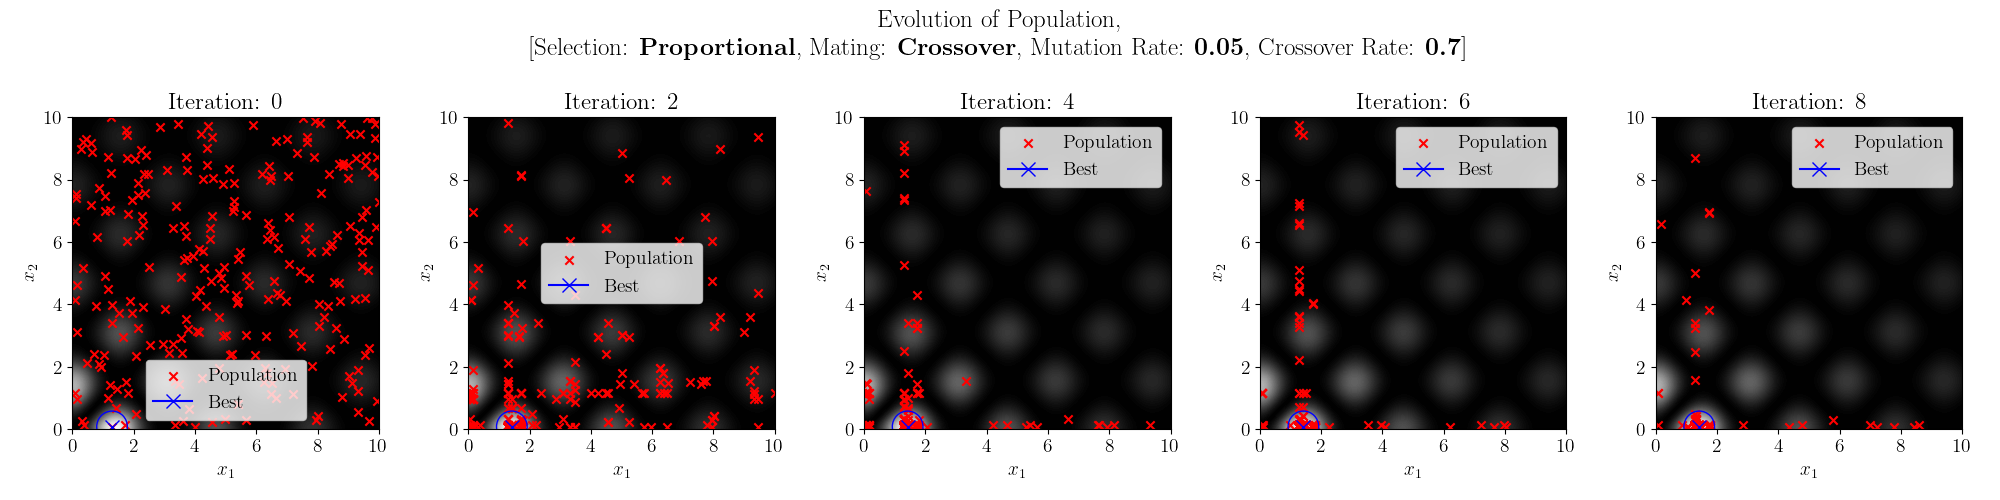
\includegraphics[width=\textwidth]{../figures/KBF/10_iters/Proportional/Crossover/0.05_0.7_Population.png}
        \caption{Mutation Procedure: Crossover}
        \label{fig:CGA_flowchart_proportional_crossover}
    \end{subfigure}
    \begin{subfigure}{0.85\textwidth}
        \centering
        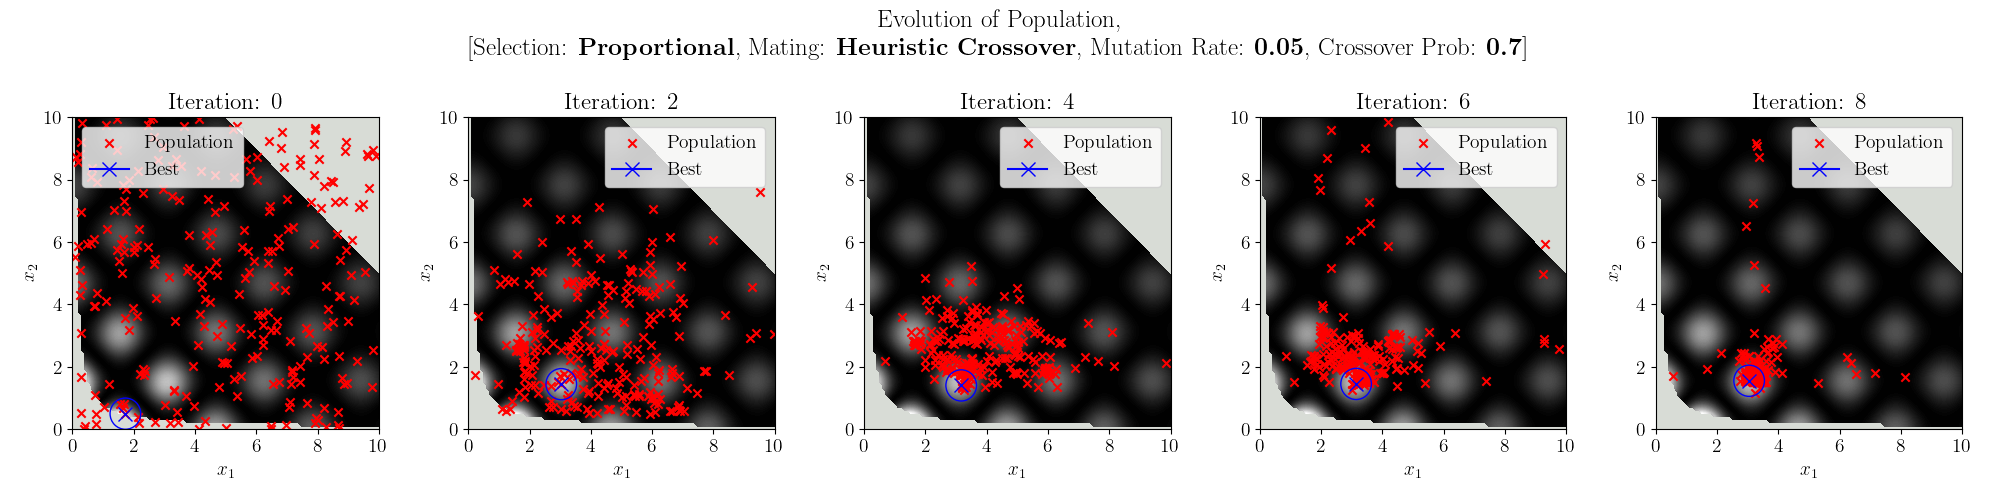
\includegraphics[width=\textwidth]{../figures/KBF/10_iters/Proportional/Heuristic Crossover/0.05_0.7_Population.png}
        \caption{Mutation Procedure: Heuristic Crossover}
        \label{fig:CGA_flowchart_proportional_Heuristic Crossover}
    \end{subfigure}
    \captionsetup{justification=centering}
    \caption{Evolution of the CGA population over 8 iterations using proportional selection. Proportional selection proved to be a somewhat effective selection method. However, it was not chosen over tournament selection as the primary selection method for the reasons outlined in Section \ref{sec:CGA_selection_mutation}.}
    \label{fig:CGA_flowchart_proportional}
\end{figure}

% \begin{figure}[H]
%     \centering
%     \begin{subfigure}{0.85\textwidth}
%         \centering
%         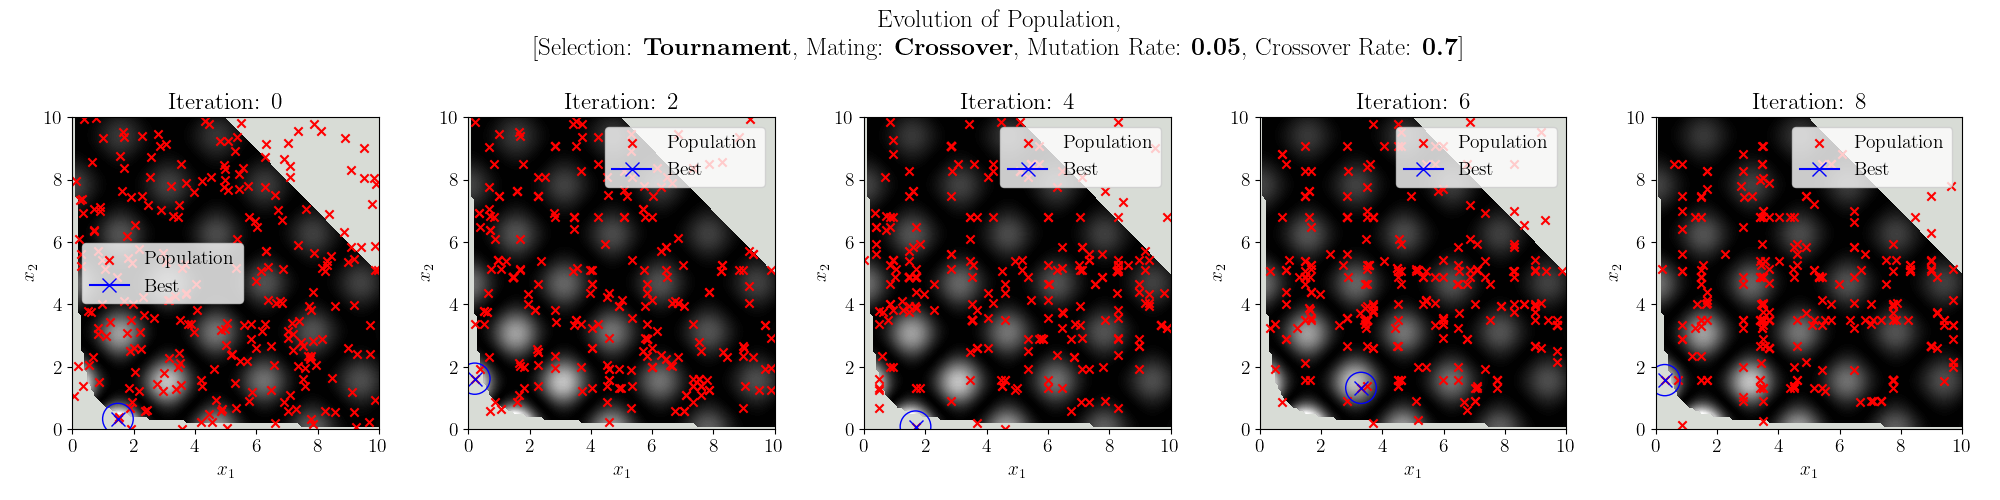
\includegraphics[width=\textwidth]{../figures/KBF/10_iters/Tournament/Crossover/0.05_0.7_Population.png}
%         \caption{Mutation Procedure: Crossover}
%         \label{fig:CGA_flowchart_tournament_crossover}
%     \end{subfigure}
%     \begin{subfigure}{0.85\textwidth}
%         \centering
%         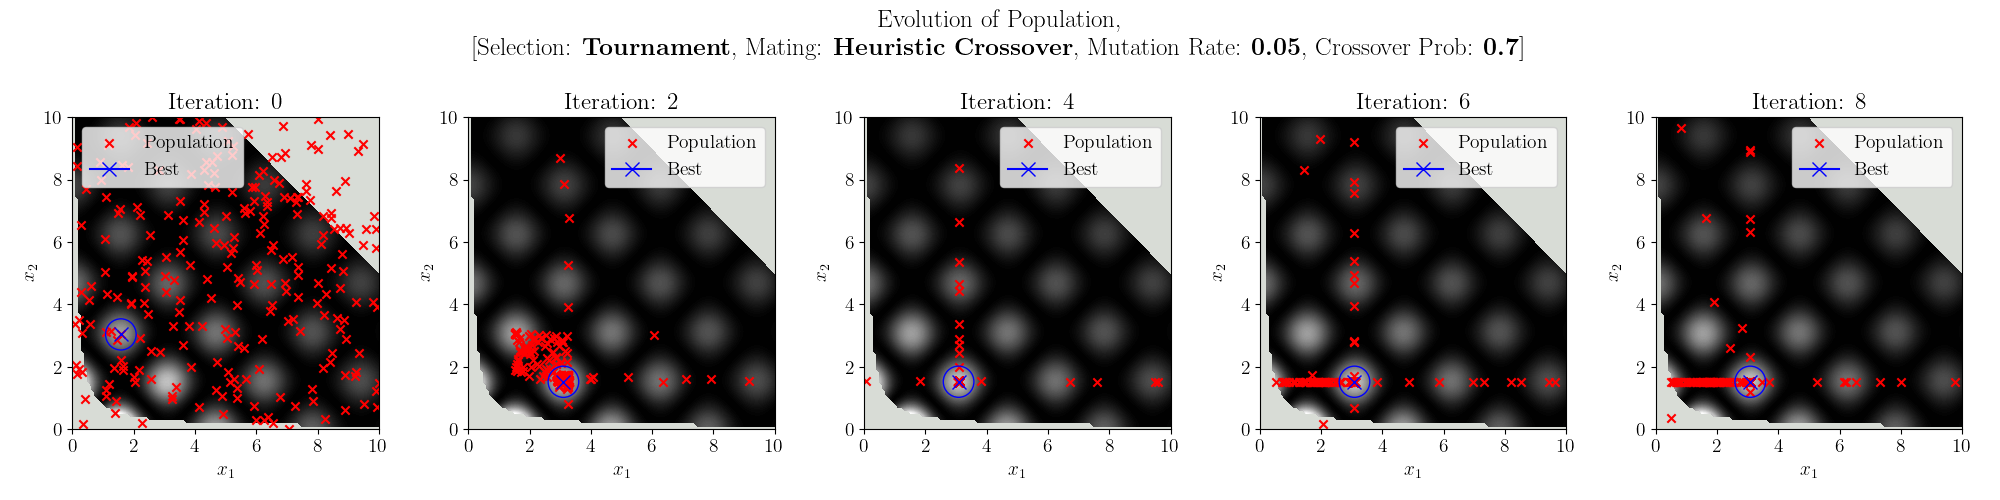
\includegraphics[width=\textwidth]{../figures/KBF/10_iters/Tournament/Heuristic Crossover/0.05_0.7_Population.png}
%         \caption{Mutation Procedure: Heuristic Crossover}
%         \label{fig:CGA_flowchart_tournament_Heuristic Crossover}
%     \end{subfigure}
%     \captionsetup{justification=centering}
%     \caption{Evolution of the CGA population over 8 iterations using tournament selection. Tournament selection proved to be the most effective selection method, when compared to Proportional Selection and Stochastic Remainder Selection without Replacement (SRS), as discussed in \ref{sec:CGA_selection_mutation}.}
%     \label{fig:CGA_flowchart_tournament}
% \end{figure}

\begin{figure}[H]
    \centering
    \begin{subfigure}{0.85\textwidth}
        \centering
        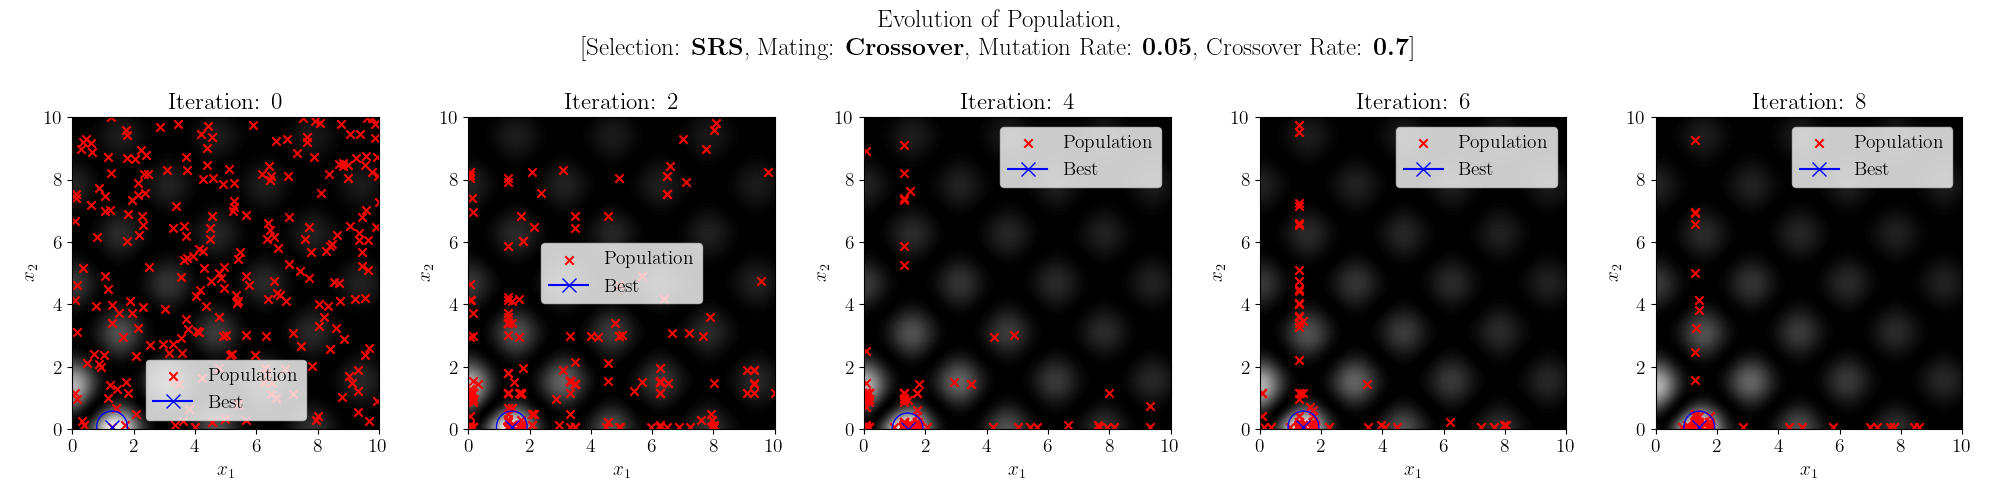
\includegraphics[width=\textwidth]{../figures/KBF/10_iters/SRS/Crossover/0.05_0.7_Population.png}
        \caption{Mutation Procedure: Crossover}
        \label{fig:CGA_flowchart_SRS_crossover}
    \end{subfigure}
    \begin{subfigure}{\textwidth}
        \centering
        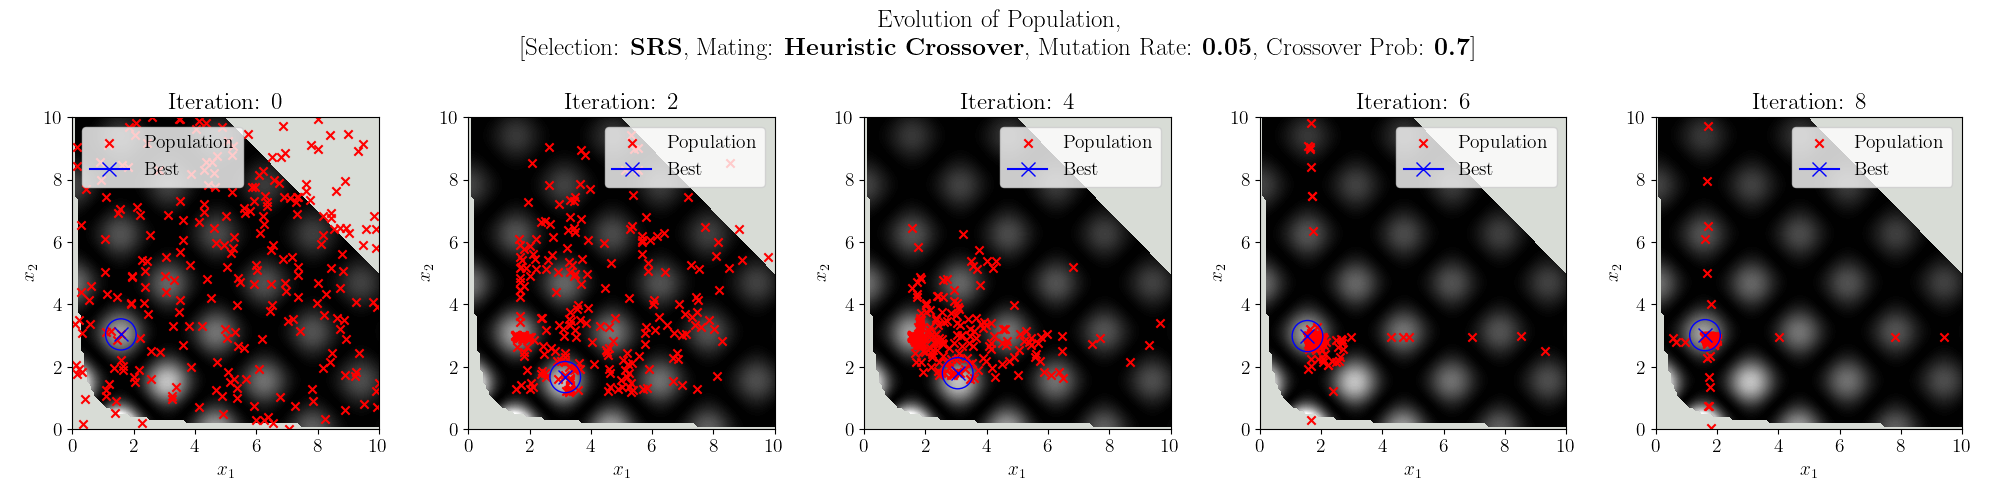
\includegraphics[width=0.85\textwidth]{../figures/KBF/10_iters/SRS/Heuristic Crossover/0.05_0.7_Population.png}
        \caption{Mutation Procedure: Heuristic Crossover}
        \label{fig:CGA_flowchart_SRS_Heuristic Crossover}
    \end{subfigure}
    \captionsetup{justification=centering}
    \caption{Evolution of the CGA population over 8 iterations using stochastic remainder selection without replacement (SRS). SRS proved to be the second most effective selection method, when compared to Proportional Selection and Tournament Selection, as discussed in \ref{sec:CGA_selection_mutation}.}
    \label{fig:CGA_flowchart_SRS}
\end{figure}

\subsection{Supplementary Results regarding PT Tuning}

\begin{table}[H]
    \centering
    \begin{tabular}{|*{5}{c|}}
        \hline
        \multirow{3}{*}{Exchange Procedure} & \multirow{3}{*}{\shortstack{Exchange\\Parameter}} & \multirow{3}{*}{Power Term} & \multirow{3}{*}{Final Avg. Fitness} & \multirow{3}{*}{Final Min. Fitness} \\
        & & & & \\
        & & & & \\
        \hline
        Periodic & \multirow{3}{*}{0.1} & 1 & -0.195696325 & -0.271773819 \\
        & & 3\cellcolor{lightgray} & -0.195696325\cellcolor{lightgray} & -0.271773819\cellcolor{lightgray} \\
        & & 5\cellcolor{gray} & -0.190261962\cellcolor{gray} & -0.325543757\cellcolor{gray} \\
        \cline{2-5}
        & \multirow{3}{*}{0.3} & 1 & -0.182369994 & -0.346578069 \\
        & & 3\cellcolor{lightgray} & -0.182369994\cellcolor{lightgray} & -0.346578069\cellcolor{lightgray} \\
        & & 5\cellcolor{gray} & -0.183774281\cellcolor{gray} & -0.341275246\cellcolor{gray} \\
        \cline{2-5}
        & \multirow{3}{*}{0.5} & 1 & -0.158484931 & -0.267351197 \\
        & & 3\cellcolor{lightgray} & -0.158484931\cellcolor{lightgray} & -0.267351197\cellcolor{lightgray} \\
        & & 5\cellcolor{gray} & -0.171493053\cellcolor{gray} & -0.341275246\cellcolor{gray} \\
        \hline
        Stochastic & \multirow{3}{*}{0.1} & 1 & -0.181921769 & -0.33399822 \\
        & & 3\cellcolor{lightgray} & -0.181921769\cellcolor{lightgray} & -0.33399822\cellcolor{lightgray} \\
        & & 5\cellcolor{gray} & -0.192349346\cellcolor{gray} & -0.33399822\cellcolor{gray} \\
        \cline{2-5}
        & \multirow{3}{*}{0.3} & 1 & -0.209998474 & -0.347740414 \\
        & & 3\cellcolor{lightgray} & -0.209998474 \cellcolor{lightgray}& -0.347740414\cellcolor{lightgray} \\
        & & 5\cellcolor{gray} & -0.202770259\cellcolor{gray} & -0.345528224\cellcolor{gray} \\
        \cline{2-5}
        & \multirow{3}{*}{0.5} & 1 & -0.206847914 & -0.357649754 \\
        & & 3\cellcolor{lightgray} & -0.206847914\cellcolor{lightgray} & -0.357649754\cellcolor{lightgray} \\
        & & 5\cellcolor{gray} & -0.202650445\cellcolor{gray} & -0.354243287\cellcolor{gray} \\
        \hline
    \end{tabular}
    \caption{Raw results from an initial exploration of the exchange procedure, exchange parameter, and power term hyperparameters within PT. Presented as the final fitness values of the PT population after 100 iterations. Here, minimum fitness refers to the fitness of the best (feasible) solution across all chains.}
    \label{tab:exchange_results}
\end{table}

\begin{figure}[H]
    \centering
    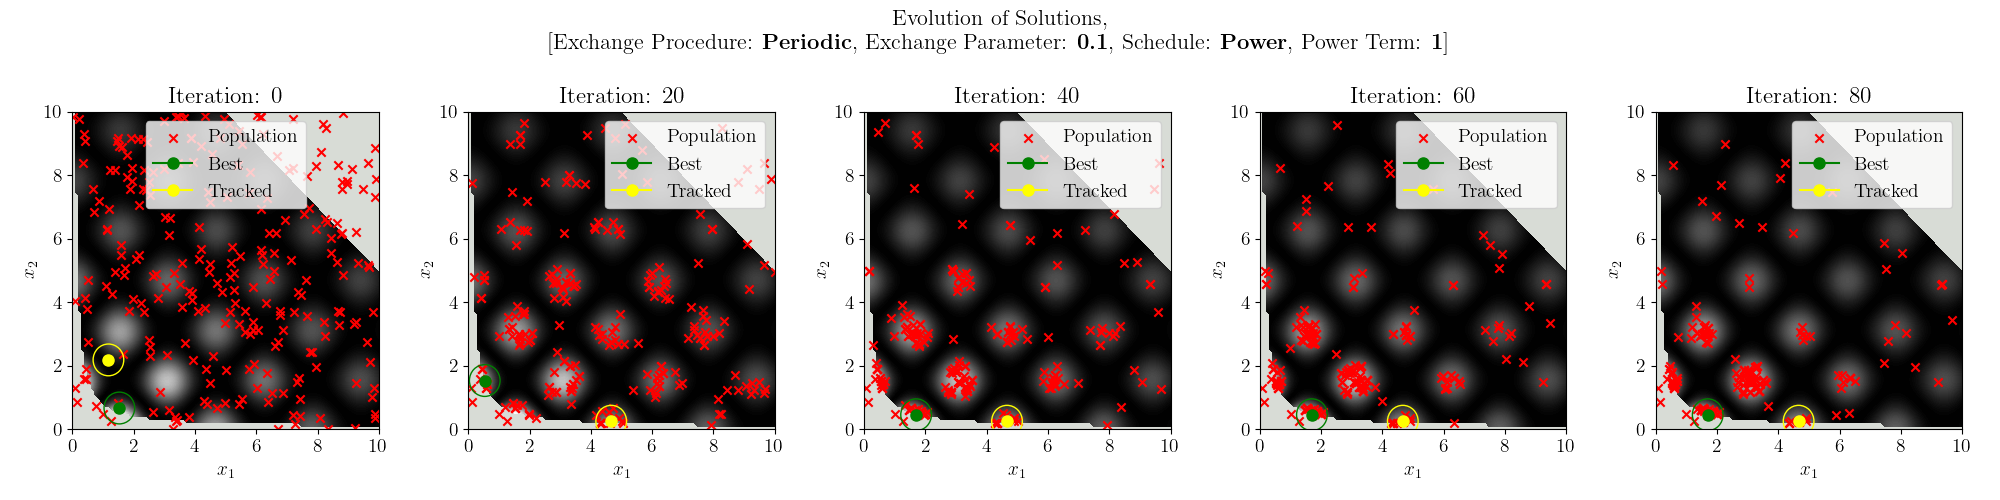
\includegraphics[width=0.85\textwidth]{../figures/KBF/100_iters/Periodic/Power/0.1_1_Solutions.png}
    \captionsetup{justification=centering}
    \caption{Evolution of the solutions across all chains over 100 iterations using periodic replica exchange and a uniform temperature scheduling, (power term of 1). Here, replica exchange occurs every 10\% of the time, (exchange parameter set to 0.1).}
    \label{fig:PeriodicApp}
\end{figure}

\begin{figure}[H]
    \centering
    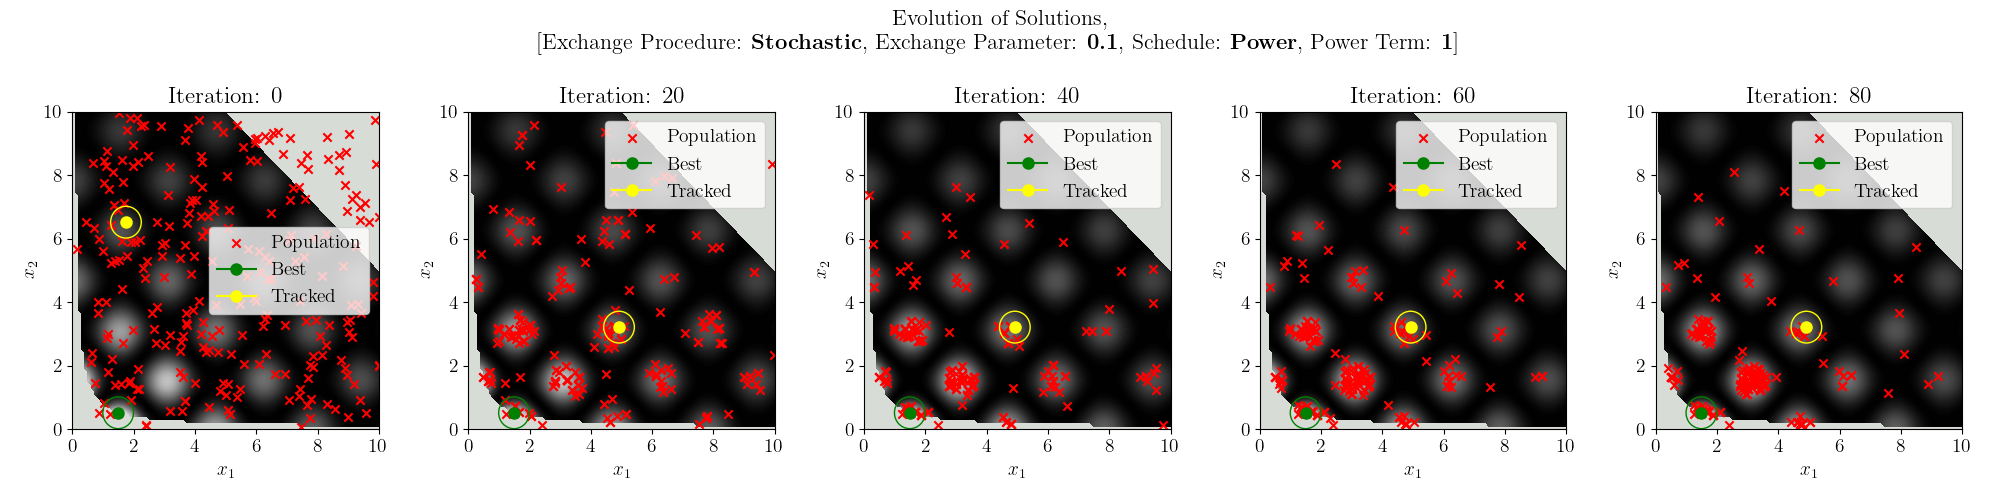
\includegraphics[width=0.85\textwidth]{../figures/KBF/100_iters/Stochastic/Power/0.1_1_Solutions.png}
    \captionsetup{justification=centering}
    \caption{Evolution of the solutions across all chains over 100 iterations using stochastic replica exchange and a uniform temperature scheduling, (power term of 1). Here, replica exchange occurs with a probability of 10\%.}
    \label{fig:StochasticApp}
\end{figure}

\end{document}


